\documentclass[a4paper, 12pt]{article}
\usepackage[utf8]{inputenc}
\usepackage[english,russian]{babel}
\usepackage[warn]{mathtext}
\usepackage{graphicx}
\usepackage{float}
\restylefloat{table}
\usepackage{amsmath}
\usepackage{floatflt}
\usepackage[T2A]{fontenc}
\usepackage[left=20mm, top=20mm, right=20mm, bottom=20mm, footskip=10mm]{geometry}

\tolerance 1414
\hbadness 1414
\emergencystretch 1.5em
\hfuzz 0.3pt        % размер максимального переполнения без warning'a
\widowpenalty=10000 % запрещает одиночную строку абзаца в начале страницы
\vfuzz \hfuzz
\raggedbottom       % если на странице мало содержимого, добавить пустое место в конце, а не в середине страницы



\begin{document}

\begin{titlepage}
	\centering
	\vspace{5cm}
	{\scshape\LARGE московский физико-технический институт (национальный исследовательский университет) \par}
	\vspace{6cm}
	{\scshape\Large Лабораторная работа 3.3.6 \par}
	{\huge\bfseries Влияние магнитного поля на проводимость полупроводников \par}
	\vspace{1cm}
	\vfill
\begin{flushright}
	{\large Б03-102}\par
	\vspace{0.3cm}
	{\LARGE Куланов Александр}
\end{flushright}
	

	\vfill


	Долгопрудный, 2022 г.
\end{titlepage}

\begin{itemize}
	\item \textbf{Цель работы:} Измерение влияния магнитного поля на полупроводники
    \item \textbf{В работе используются:} Стабилизированный источник постоянного тока и напряжения, электромагнит, цифровой вольтметр, aмперметр, миллиамперметр, реостат, измеритель магнитной индукции III1-10, образцы (InSb) монокристаллического антимонида индия n-типа
    
\end{itemize}

\section{Описание установки}
\begin{figure}[H]
    \centering
    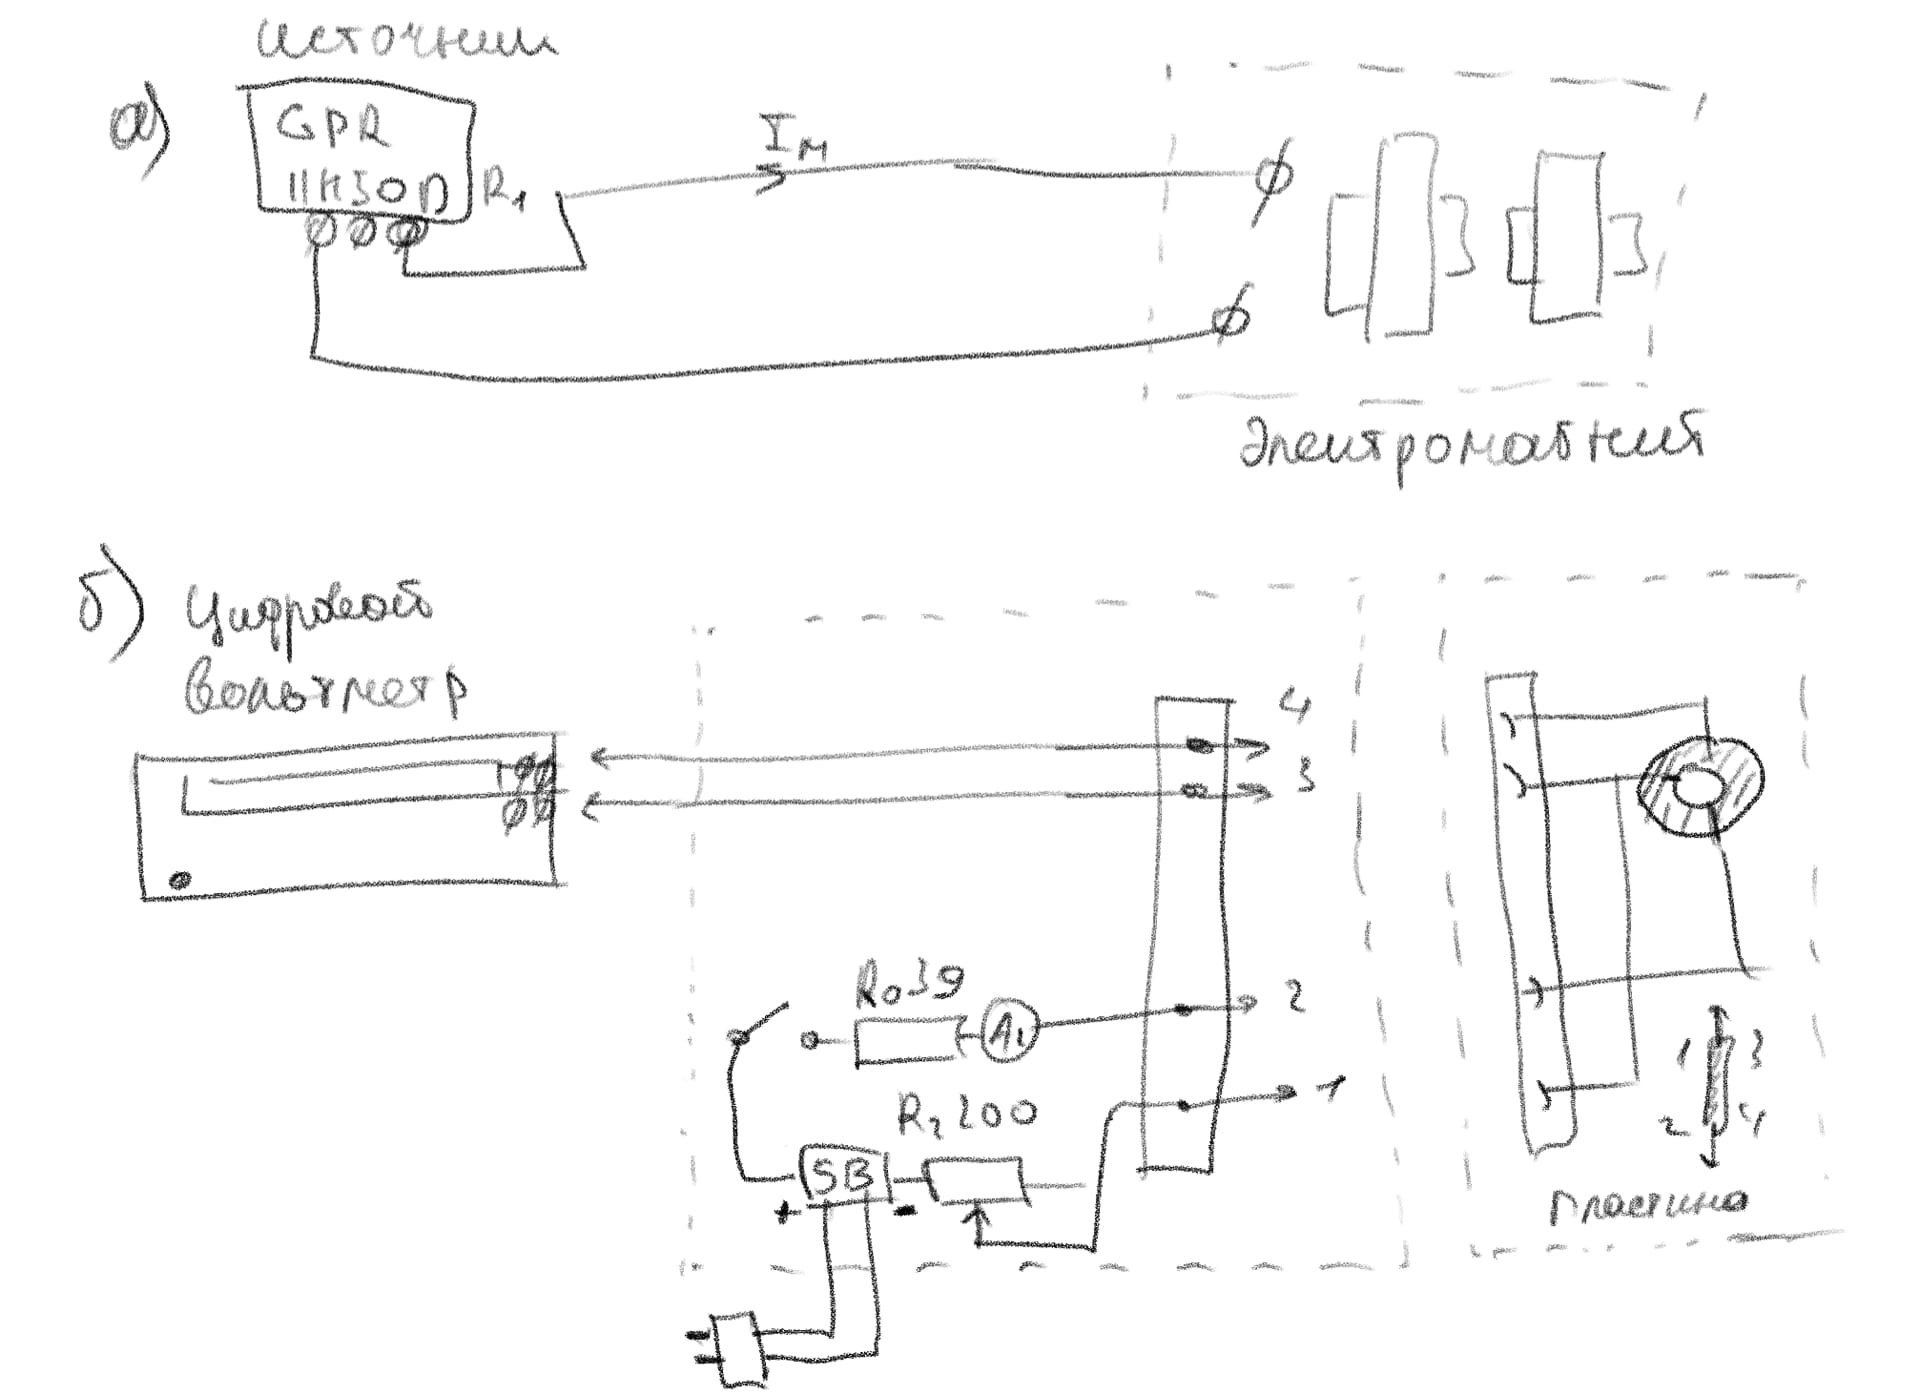
\includegraphics[width=0.7\textwidth]{set}
    \caption{Схема установки}
    \label{fig:set}
\end{figure}

В зазоре электромагнита создаётся постоянное магнитное поле. Ток питания магнита подаётся от источника постоянного напряжения GPR-11H30D, регулируется ручками управления источника $\left(R_{1}\right)$ и измеряется амперметром источника $A_{1}$. Магнитная индукция в зазоре электромагнита определяется при помощи измерителя магнитной индукции Ш1-10 (описание прибора расположено на установке).

Образец в форме кольца (диск Корбино) или пластинки, смонтированный в специальном держателе, подключается к источнику постоянного напряжения 5 В. При замыкании ключа К сквозь образец течёт ток, величина которого измеряется миллиамперметром $A_{2}$ и регулируется реостатом $R_{2}$ Балластное сопротивление $R_{0}$ ограничивает ток через образец. Измеряемое напряжение подаётся на вход цифрового вольтметра $\mathrm{B} 7-78 / 1$

\section{Теоретические сведения}
\section{Обработка результатов}
\subsection*{Калибровка магнита}
По данным из таблицы \ref{tab:cal} построим график зависимости $B(I_m)$
\begin{table}[]
	\centering
	\begin{tabular}{|c|c|}
	\hline
	\textbf{B, мТл} & \textbf{I, А} \\ \hline
	42              & 0.04          \\ \hline
	95.2            & 0.10          \\ \hline
	178.5           & 0.18          \\ \hline
	277             & 0.29          \\ \hline
	333             & 0.39          \\ \hline
	365             & 0.48          \\ \hline
	378             & 0.55          \\ \hline
	\end{tabular}
	\caption{Зависимость $B(I_m)$}
	\label{tab:cal}
\end{table}
\begin{figure}[H]
    \centering
    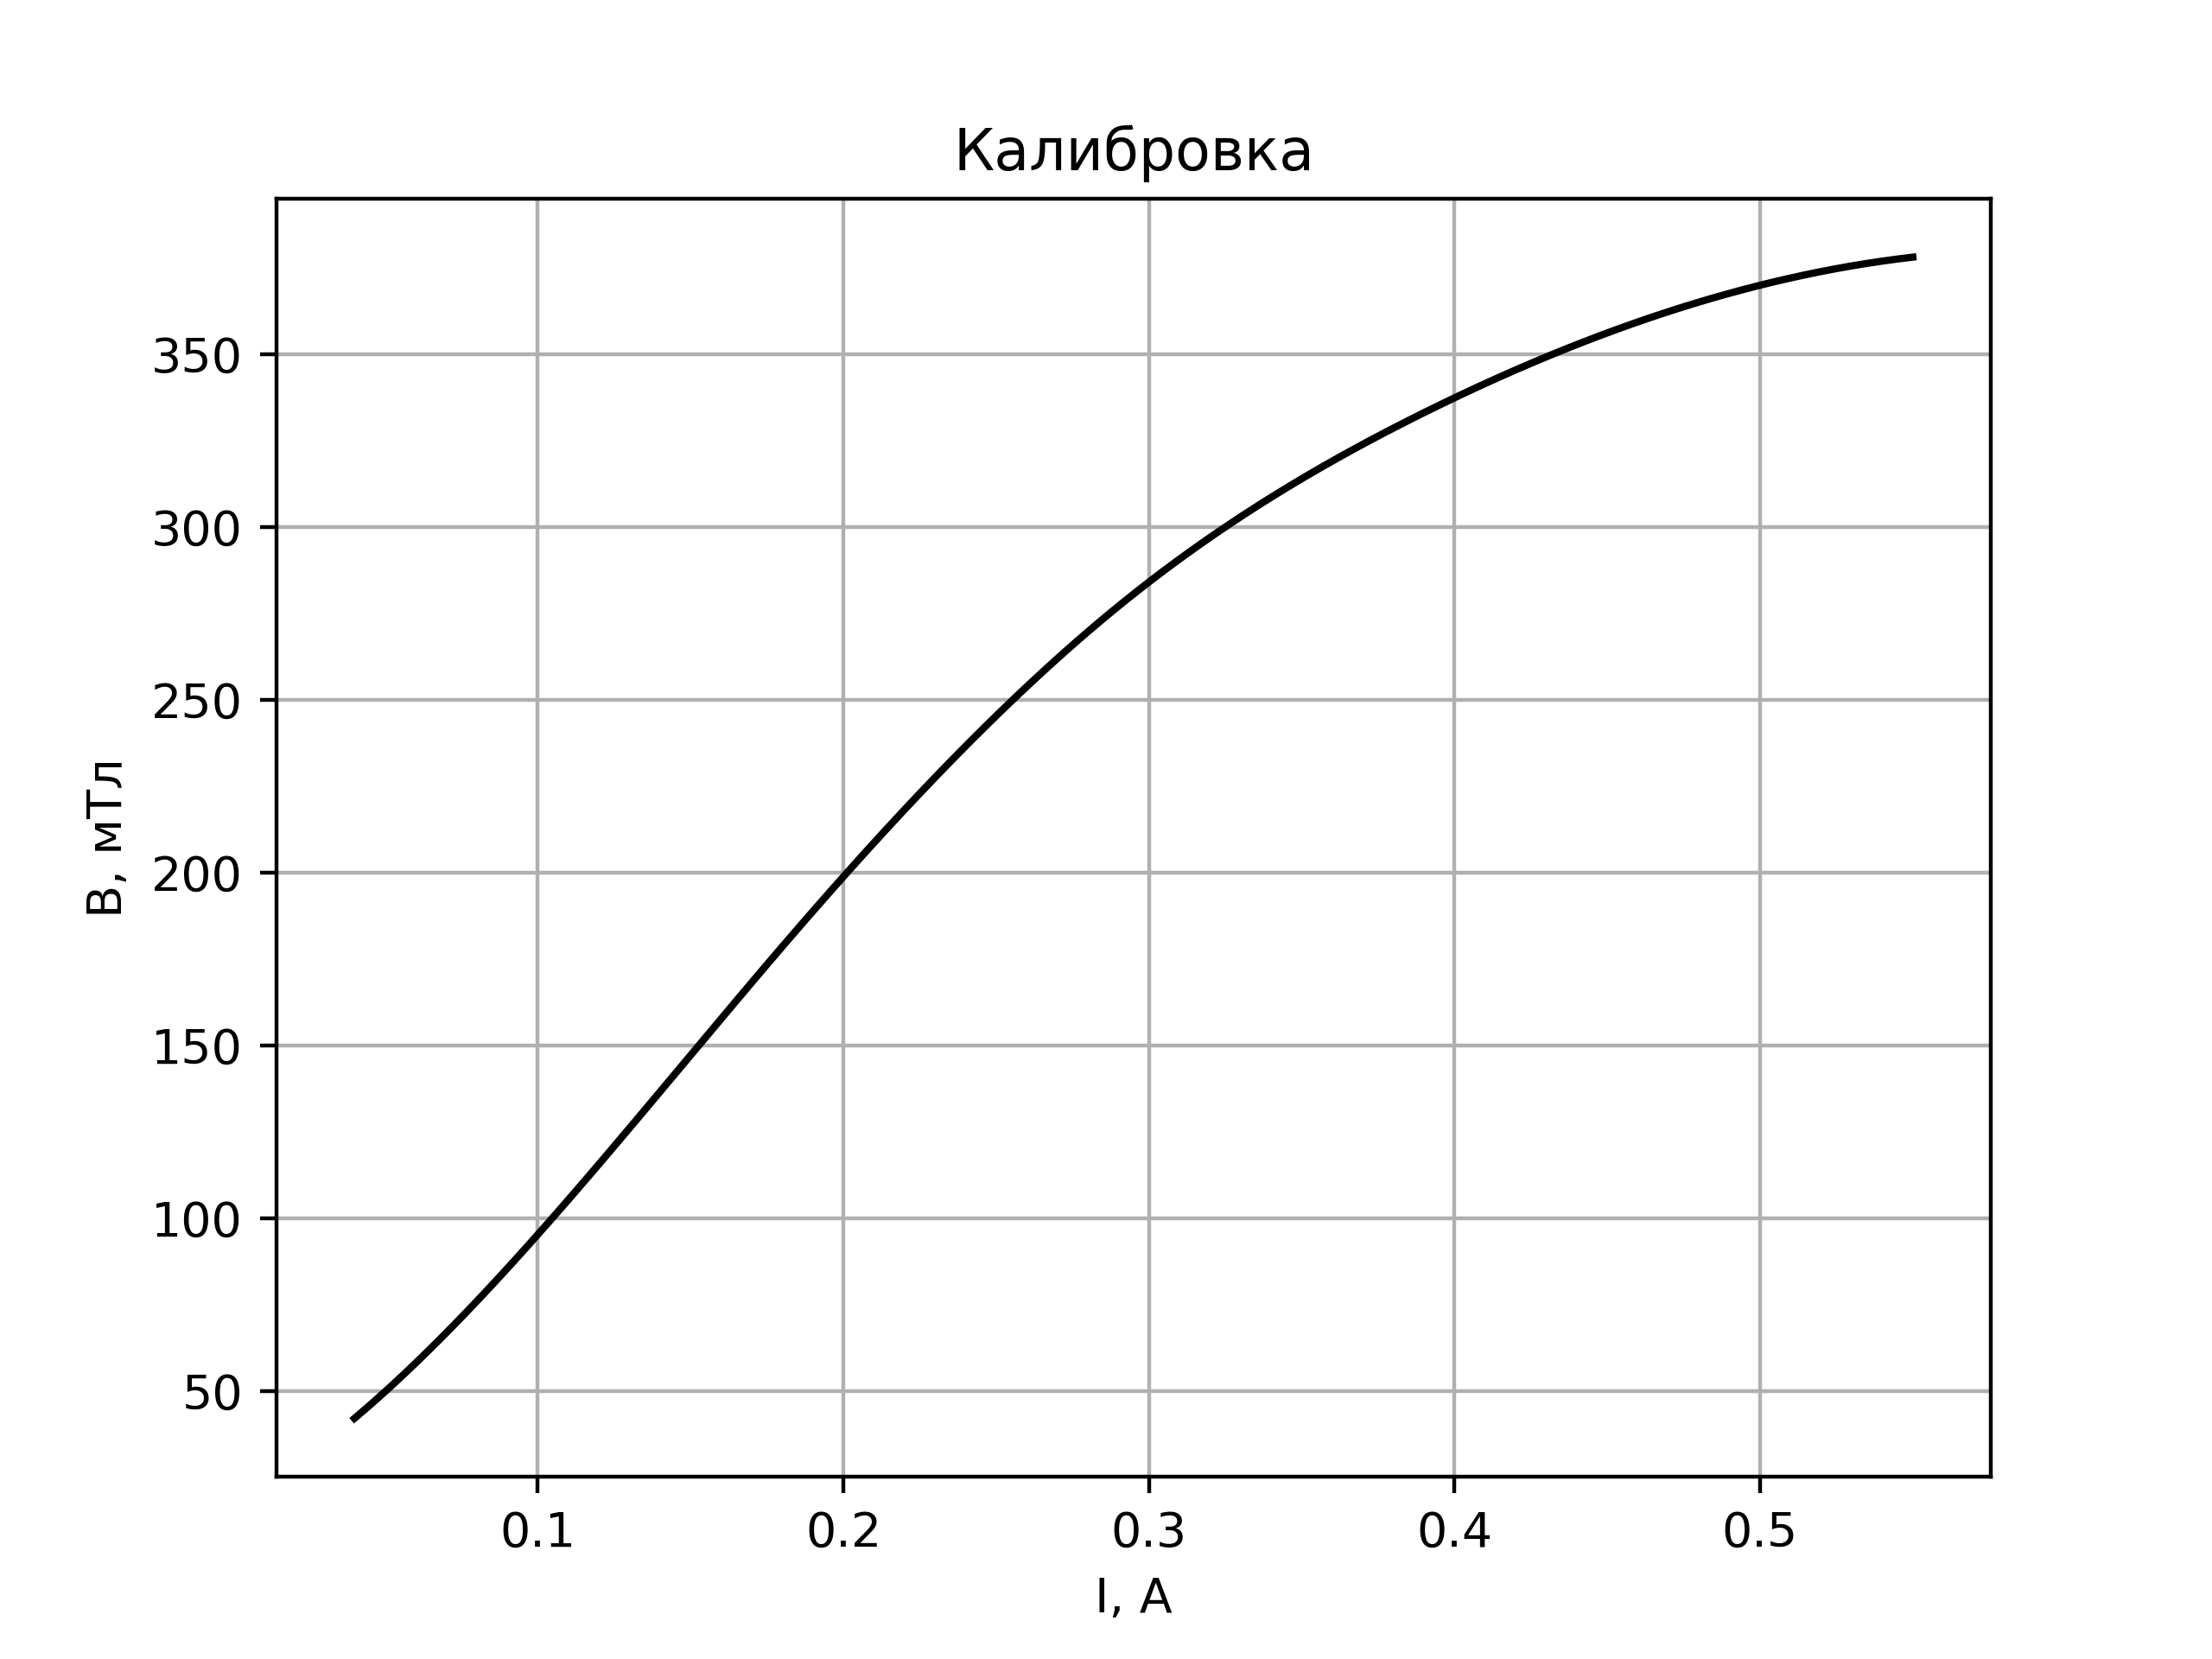
\includegraphics[width=1\textwidth]{calibration.png}
    \caption{Зависимость $B(I_m)$}
    \label{fig:cal}
\end{figure}

\subsection*{Пластинка}

Полученные данные занесем в таблицу \ref{tab:plate}

\begin{table}[H]
\centering
\begin{tabular}{|cc|cc|}
\hline
\multicolumn{2}{|c|}{\textbf{Перпендикулярно}} & \multicolumn{2}{c|}{\textbf{Параллельно}}  \\ \hline
\multicolumn{1}{|c|}{U, мВ}       & I, А       & \multicolumn{1}{c|}{U, мВ} & I, А \\ \hline
\multicolumn{1}{|c|}{0.688}       & 0          & \multicolumn{1}{c|}{0.688} & 0    \\ \hline
\multicolumn{1}{|c|}{0.722}       & 0.06       & \multicolumn{1}{c|}{0.701} & 0.06 \\ \hline
\multicolumn{1}{|c|}{0.789}       & 0.11       & \multicolumn{1}{c|}{0.729} & 0.11 \\ \hline
\multicolumn{1}{|c|}{0.966}       & 0.20       & \multicolumn{1}{c|}{0.800} & 0.20 \\ \hline
\multicolumn{1}{|c|}{1.193}       & 0.30       & \multicolumn{1}{c|}{0.887} & 0.31 \\ \hline
\multicolumn{1}{|c|}{1.324}       & 0.42       & \multicolumn{1}{c|}{0.940} & 0.42 \\ \hline
\multicolumn{1}{|c|}{1.375}       & 0.5        & \multicolumn{1}{c|}{0.965} & 0.5  \\ \hline
\multicolumn{1}{|c|}{1.414}       & 0.57       & \multicolumn{1}{c|}{0.978} & 0.56 \\ \hline
\multicolumn{1}{|c|}{1.416}       & 0.58       & \multicolumn{1}{c|}{0.980} & 0.57 \\ \hline
\end{tabular}
\caption{Зависимости $U(I)$}
\label{tab:plate}
\end{table}
Найдем теперь $B^2$ и $R$, учитывая, что ток через образец в обоих случаях 10 мА и нанесем результат на график \ref{fig:b2}

\subsection*{Диск Корбино}
Полученные данные занесем в таблицу:
\begin{table}[H]
	\centering
	\begin{tabular}{|c|c|}
	\hline
	U, мВ & I, А \\ \hline
	0.712 & 0    \\ \hline
	0.794 & 0.06 \\ \hline
	1.016 & 0.12 \\ \hline
	1.527 & 0.20 \\ \hline
	2.319 & 0.30 \\ \hline
	2.940 & 0.41 \\ \hline
	3.199 & 0.49 \\ \hline
	3.356 & 0.55 \\ \hline
	3.409 & 0.58 \\ \hline
	\end{tabular}
	\caption{Данные для диска Корбино}
	\label{tab:disk}
	\end{table}
Аналогично пластике, найдем $B^2$ и $R$, но ток в данном случае 23,5 А, нанесем результаты на график \ref{fig:b2}

\begin{figure}[H]
    \centering
    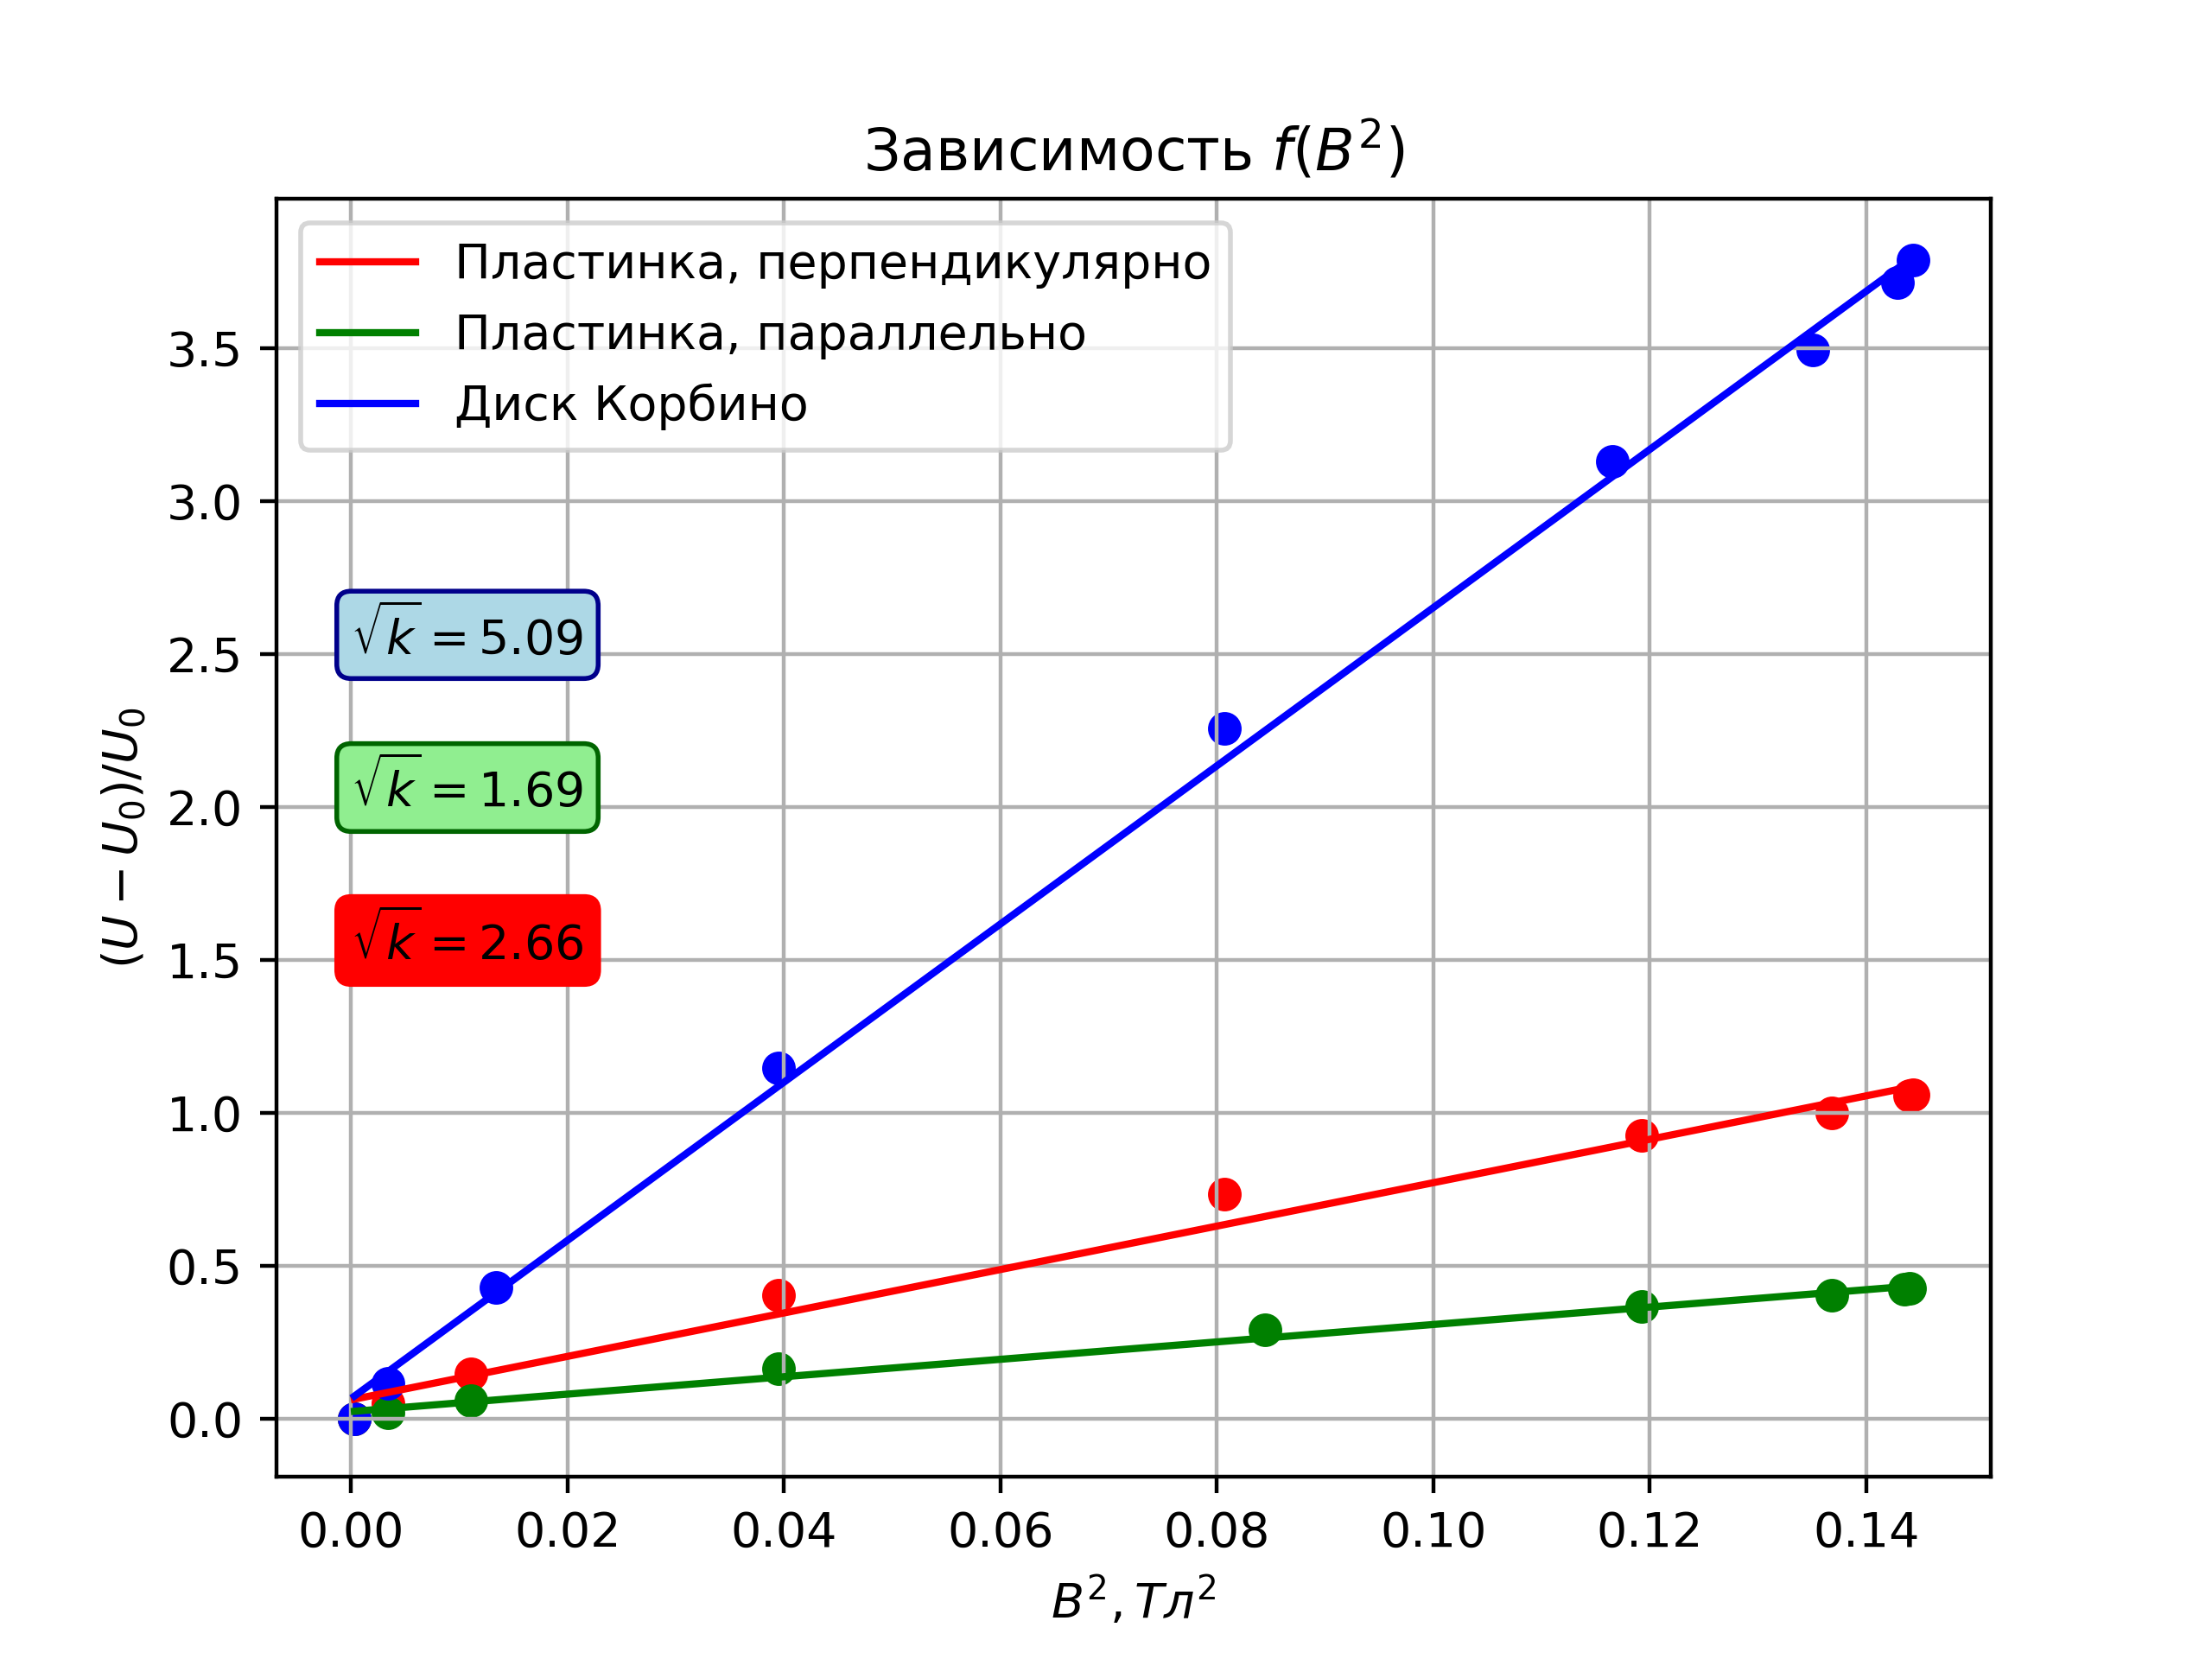
\includegraphics[width=1\textwidth]{B2.png}
    \caption{Зависимость $R(B^2)$}
    \label{fig:b2}
\end{figure}



\section{Приложение}

\end{document}